\documentclass{article}

\usepackage[margin=2cm]{geometry}
\usepackage{ctex}
\usepackage[hidelinks]{hyperref}
\usepackage{url}
% \hypersetup{colorlinks=}
\usepackage{fancyvrb}

\usepackage{xcolor}
\definecolor{theme}{HTML}{3755BE}
\definecolor{dark}{HTML}{030719}

\usepackage{graphicx}

\usepackage{amsmath,amssymb}

\title{Python预习简介}
\author{TechX机器学习课程学术团队}
\date{2021年6月}

\begin{document}

\maketitle

\section{为什么要用Python}
因为Python是一门非常简单易懂,而广泛使用的语言。
现在机器学习界大部分前沿学者都在使用Python编写,也因此有很多好用而强大的Python机器学习模块。
所以在开始学习机器学习的旅程之前,我们会先通过预习材料来学习一下Python的基础。

\section{使用Python}
TechX通过Jupyter Hub给学员提供了在线运行Python的计算资源。请访问我们的Jupyter Hub网址 \url{https://mlds.xa2021.xacademy.cc/}。

\vspace*{0.3cm}\centerline{\noindent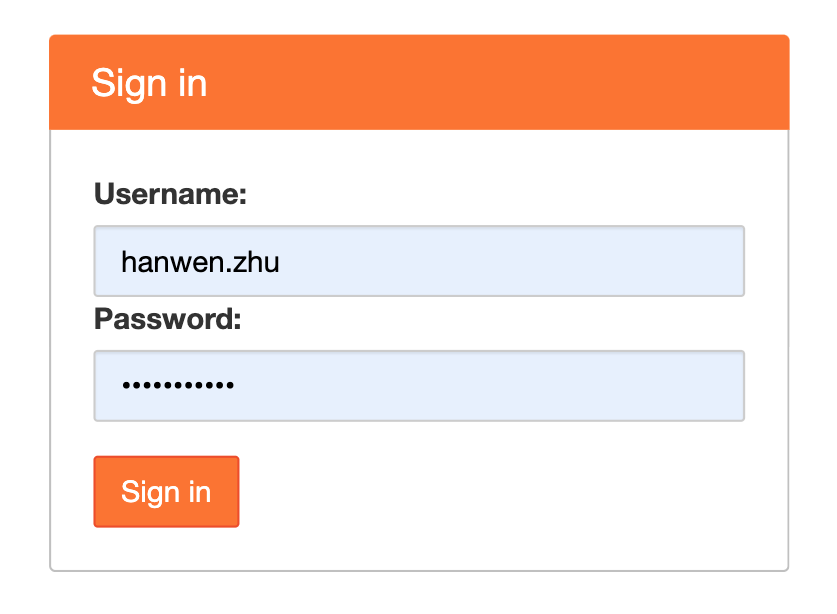
\includegraphics[width=0.5\textwidth]{hub-signin.png}}

在初次登录时请使用用户名 \texttt{名拼音.\hspace*{0cm}姓拼音},例如:\texttt{hanwen.zhu}。接着请输入你想要设置的密码,但\textbf{请记住这个密码,这个密码就是你今后登录Jupyter Hub的密码}。

进入之后,可以在右上角选择Upload上传本地的Notebook文件,或者选择New $\rightarrow$ Notebook: Python 3来新建一个Jupyter代码文件,如图:

\vspace*{0.3cm}\centerline{\noindent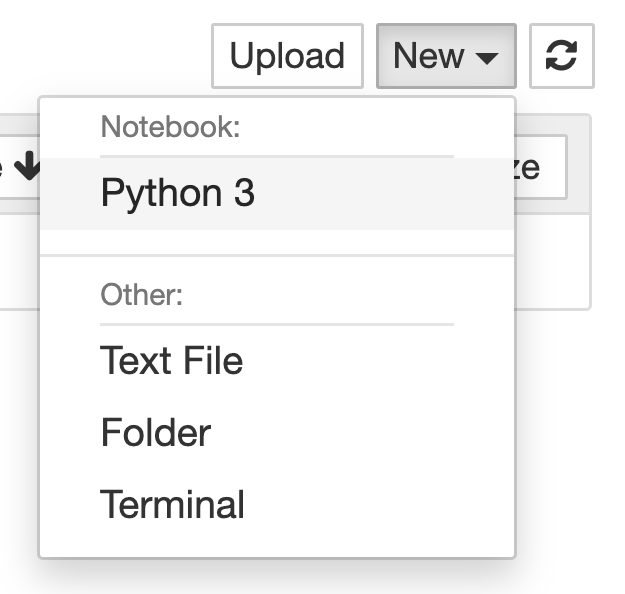
\includegraphics[width=0.2\textwidth]{new-ipynb.png}}

这时,你会来到一个新的Notebook文件中。你可以点击上方的Untitled来给自己的文件重命名:

\vspace*{0.3cm}\centerline{\noindent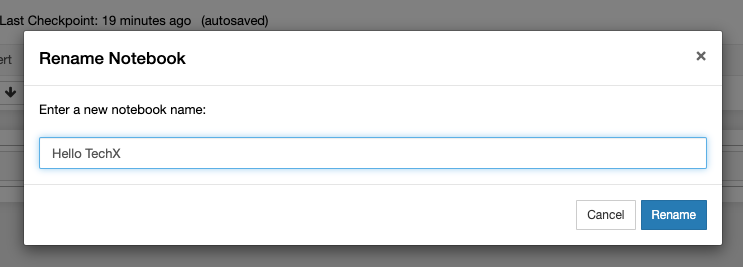
\includegraphics[width=0.8\textwidth]{ipynb-rename.png}}

然后就可以在Notebook里面写代码了!你可以先试一下最基础的\texttt{1 + 1}和\texttt{print}命令:

\vspace*{0.3cm}\centerline{\noindent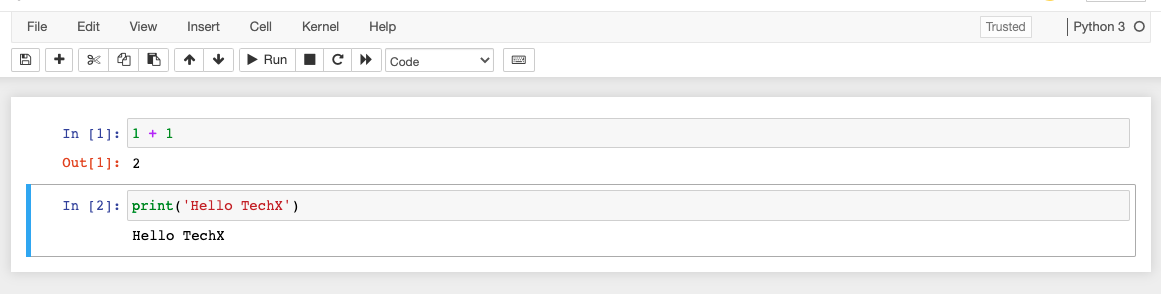
\includegraphics[width=0.8\textwidth]{ipynb-code.png}}

在每个框里面写好代码,点击上面的“$\blacktriangleright$ Run”按钮即可运行。

Notebook文件的后缀名是\texttt{ipynb},今后的预习资料都将以Notebook形式发送,将这个文件上传到Jupyter Hub,点击文件名就可以打开运行了!

\vspace*{0.3cm}\centerline{\noindent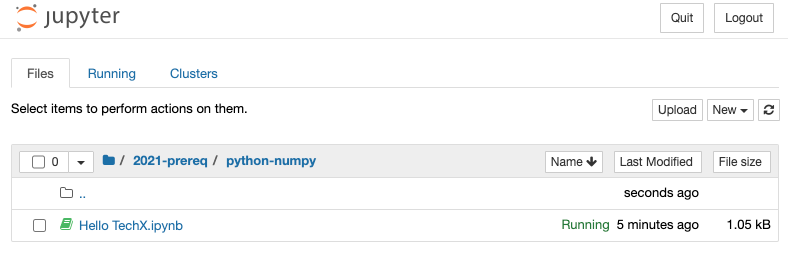
\includegraphics[width=0.8\textwidth]{ipynb-open.png}}

\emph{我们推荐使用我们的Jupyter Hub即可,不需要在自己的电脑上安装Python。但是对于想要在自己电脑上运行的学员,以下是本地运行Jupyter Notebook的教程。}

\section{(可选)本地安装Python}
TechX的机器学习课程使用的是Python 3.7及以上的版本。如果你的电脑上还没有安装Python 3.7+,可以到官网下载:

点击Python官网下载链接 \url{https://www.python.org/downloads/release/python-3711/},在页面下方选择你电脑的版本:
\begin{itemize}
\item
Windows用户请选择 Windows installer (64-bit)
\item
macOS用户选择 macOS 64-bit Intel installer
\end{itemize}
下载完成后,即可打开完成安装。Windows在安装的时候务必勾选“Add Python 3.x to PATH”。

随后在Windows中使用Win+R键打开运行,输入\texttt{cmd}进入“命令提示符”。在macOS上请打开“终端” Terminal软件。

现在你应该可以看到一个空空的窗口,输入\texttt{python}(Windows)或者\texttt{python3}(macOS)并按下回车,如果出现\texttt{>>>}就代表Python安装成功了!接着可以输入下面这个代码:\texttt{exit()}来退出。全过程如下所示,蓝色为你输入的内容,并请确保红色版本为3.7及以上:

\begin{Verbatim}[commandchars=\\\{\},xleftmargin=1.5cm]
\color{dark}$> \textcolor{theme}{python}
\color{dark}Python \textcolor{red}{3.7.11} (default, May 4 2021, 11:57:03)
\color{dark}[Clang 11.0.0 (clang-1100.0.33.17)] on darwin
\color{dark}Type "help", "copyright", "credits" or "license" for more information.
\color{dark}>>> \textcolor{theme}{1 + 1}
\color{dark}2
\color{dark}>>> \textcolor{theme}{exit()}
\color{dark}$>
\end{Verbatim}

如果安装遇到任何问题,请直接在微信上联系我们。我们随时可以为你提供详细的指导!

\section{(可选)本地安装Jupyter Notebook}
Jupyter Notebook是一个用来更方便地进行Python编程的工具,在TechX之后的学习里会使用Jupyter来进行Python编程。安装过程很简单,我们在命令提示符或者终端里继续输入如下内容,使用\texttt{pip}(Windows)或\texttt{pip3}(macOS)来安装:
\begin{Verbatim}[commandchars=\\\{\},xleftmargin=1.5cm]
\color{dark}$> \textcolor{theme}{pip install notebook}
\color{dark}Looking in indexes: https://pypi.python.org/simple
\color{dark}Collecting notebook
\color{dark}...
\color{dark}Installing collected packages: notebook
\color{dark}Successfully installed notebook-6.4.0
\end{Verbatim}

然后直接键入\texttt{jupyter notebook}命令来启动Jupyter服务器:
\begin{Verbatim}[commandchars=\\\{\},xleftmargin=1.5cm]
\color{dark}$> \textcolor{theme}{jupyter notebook}
\end{Verbatim}

这段代码会自动打开浏览器。打开的页面和Jupyter Hub相同,只是在你本地的计算机上运行的。

\end{document}
